\chapter{Numerical experiments}

% НЕ пытайся заменить \cite{TODO} на что-то осознанное, я это сделаю сам потом
Для проведения численных экспериментов был использован язык Python и общеизвестные библиотеки deep learning-a PyTorch\cite{TODO} и Torch-Lightning\cite{TODO}. Для экспериментов с pretrain моделями использовались Llama 3.2 1B, Llama 3.2 3B и Llama 3.1 8B \cite{TODO}. Для обучения моделей с нуля использовалась маленькая LLama-like модель на 150М. В качестве обучающих данных использовался датасет SlimPajama \cite{TODO}. Каждая модель обученная с нуля проходила 1.5B токенов во время обучения. После обучения модели замерялись на бенчмарках MMLU\cite{TODO}, AGIEval\cite{TODO} и SQuAD\cite{TODO}. В качестве вычислительного сетапа была доступна 1x3090 Nvidia GPU. Код обучения и замеров выложен на GitHub\cite{TODO}.

% Правь subsection если тебе они кажутся плохо написанными
\subsection{Experiments with Final Hidden States and Token Embeddings}

Для предобученных моделей семейства Llama мы будем измерять NDCG скор между logit-ами модели и разными метриками сходств. Подробна методика описана в секции \ref{final_hidden_method}. Метрику мы будем замерять на сапсемпле из валидационной части датасета SlimPajama длиной 1000 примеров. Усреднение метрики происходило по 512 токенам в промпте и 20 сгенерированным токенам.


\begin{table}[h]
    \centering
    \caption{Comparison of NDCG score across different model sizes and similarities}
    \begin{tabular}{lcccc}
    \toprule
    Model & NegEuclid & InvEuclid & Cosine & Dot \\
    \midrule
    Llama 3.2 1B & 0.921 & 0.912  & 0.952 & 1.000 \\
    Llama 3.2 3B & 0.934 & 0.926  & 0.969 & 1.000 \\
    Llama 3.1 8B & 0.120 & 0.113  & 0.093 & 0.091 \\
    \bottomrule
    \end{tabular}
    \label{tab:pretrained_last_hidden_scores}
\end{table}

Исходя из результатов таблицы \ref{pretrained_last_hidden_scores} можно сделать следующие выводы:
\begin{enumerate}
    \item Для моделей Llama 3.2 1B и Llama 3.2 3B все метрики сходства ранжируют токены очень похоже на то, как ранжируютя токены стандартными logit-ами модели. Такое поведение скорее всего обусловлено тем, что эти модели обучались авторами со связыванием весов. NDCG равный 1.0 для dot similarity это подтверждает.
    \item Модель Llama 3.1 8B обучена без связывания весов. И для нее NDCG скор для всех метрик сходства оказался крайне низким. Это говорит нам о том, что модель сама по себе не пытается приблизить финальные hidden states к наиболее вероятным токенам по какой либо метрики близости.
\end{enumerate}

Мы также обучили с нуля несколько моделей с разными вариатами LmHead-ов и замерили их качество на валидационной выборке и общепринятных бенчмарках. Подробное описание вариаций языковых голов использованных в экспериментах можно найти в секции \ref{scratch_final_hidden_info}.


\begin{table}[h]
    \centering
    \caption{Comparison of validation loss and score on benchmarks across 150M Llama-like model with different LmHead}
    \begin{tabular}{lcccc}
    \toprule
    LmHead Type & Loss $\downarrow$ & MMLU (5-shot, acc) & AGIEval (4-shot, acc) & SQuAD (1-shot, em) \\
    \midrule
    (base) LmHead           & 2.84 & 27.34  & 20.1 & 25.34 \\
    $\text{LmHead}_{tied}$  & 2.89 & 27.11  & 20.3 & 24.55 \\
    KnnHead                 & 3.01 & 26.80  & 19.9 & 25.08 \\
    \bottomrule
    \end{tabular}
    \label{tab:scratch_last_hidden_scores}
\end{table}

Исходя из результатов таблицы \ref{scratch_last_hidden_scores} можно сделать следующие выводы:
\begin{enumerate}
    \item Совокупно лучшей моделью оказалась модель с стандартной LmHead (без связывания). Однако остальные модели не разломались и показали сравнимое качество.
    \item Модели достигли адекватного для своих размерах Loss-а на валидации \cite{TODO}, что говорит нам о том, что все три модели способны обучаться ожидаемым образом.
    \item Все три модели получили качество близкое к случайному угадыванию на AGIEval. Данный бенчмарк оказался слишком сложным для моделей. Либо 4 примера во few-shot оказалось недостаточным
\end{enumerate}

% Правь subsection если тебе они кажутся плохо написанными
\subsection{Experiments with Intermediate Hidden States and Token Embeddings}

Для исследования взаимного расположения промежуточных hidden state и ембеддингов токенов мы хотим провизуализировать нормы hidden state-ов после каждого слоя модели. Для этой визуализации мы будем использовать сначала предобученную модель Llama 3.2 1B.

% todo сделай две этих картинки параллельно в одну линию через minipage
\begin{figure}[h]
    \centering
    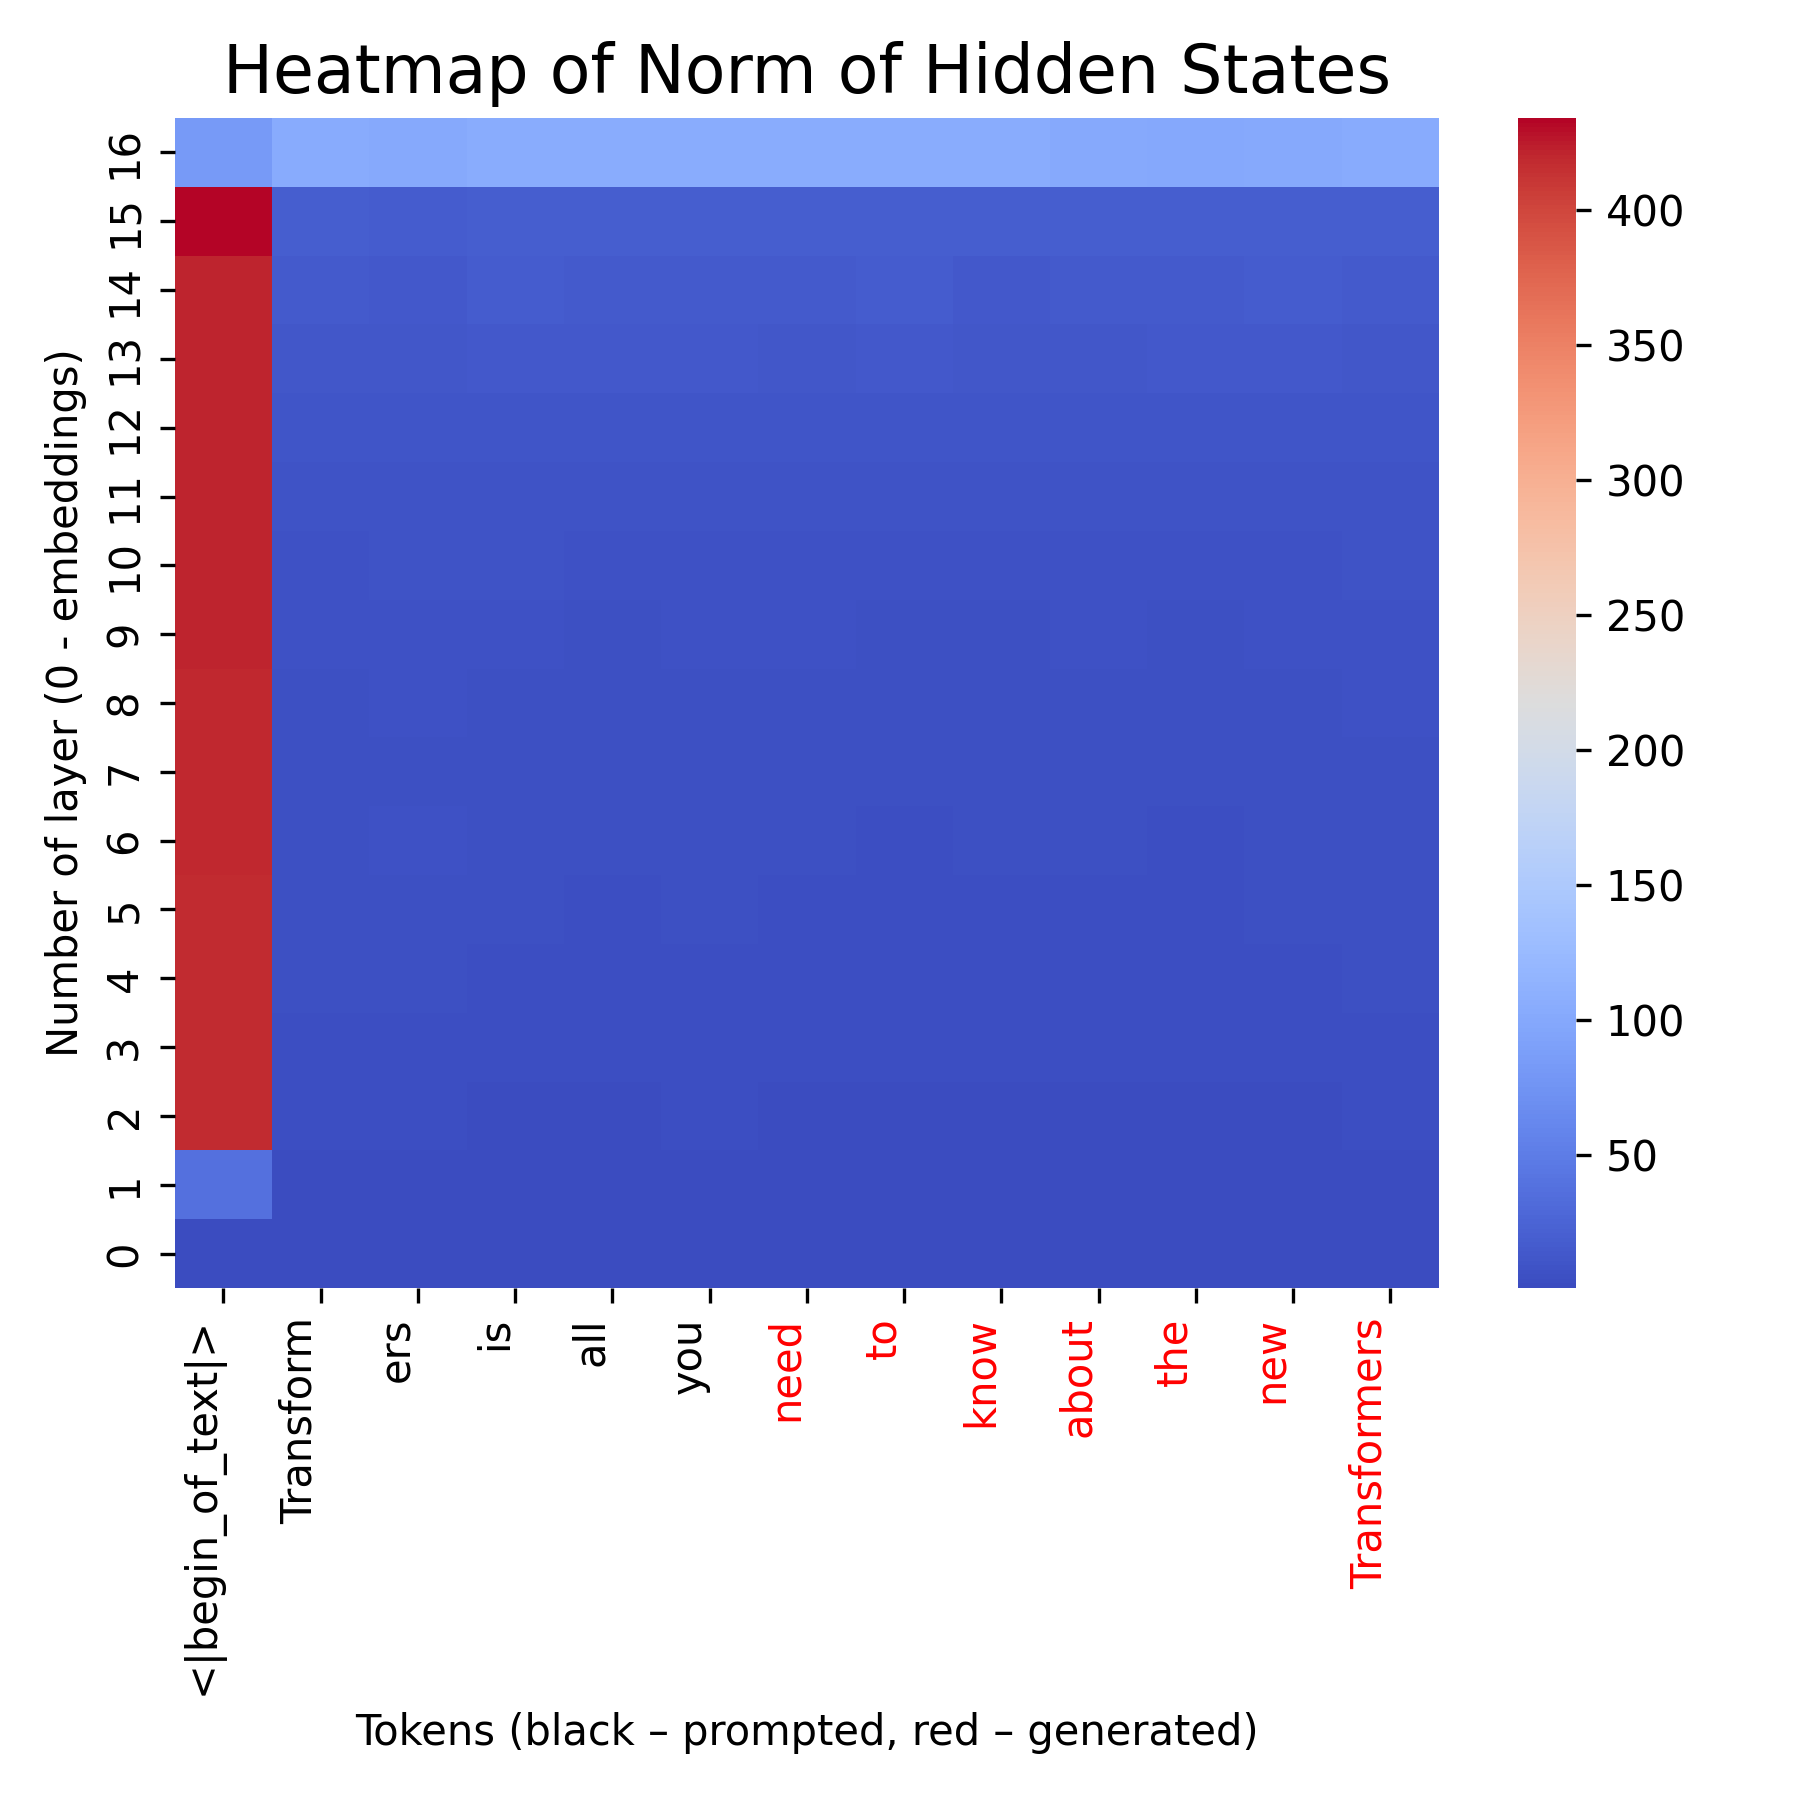
\includegraphics[width=0.5\textwidth]{images/heatmap_1b_full.png}
    \caption{Illustration of the k-nearest neighbors approach to token prediction. The final hidden state $\mathbf{h}_i^L$ (blue point) is compared to all token embeddings in the vocabulary. The closest embeddings (green points) correspond to the most likely next tokens, while distant embeddings (red points) are less probable candidates.}
    \label{fig:heatmap_1b_full}
\end{figure}

\begin{figure}[h]
    \centering
    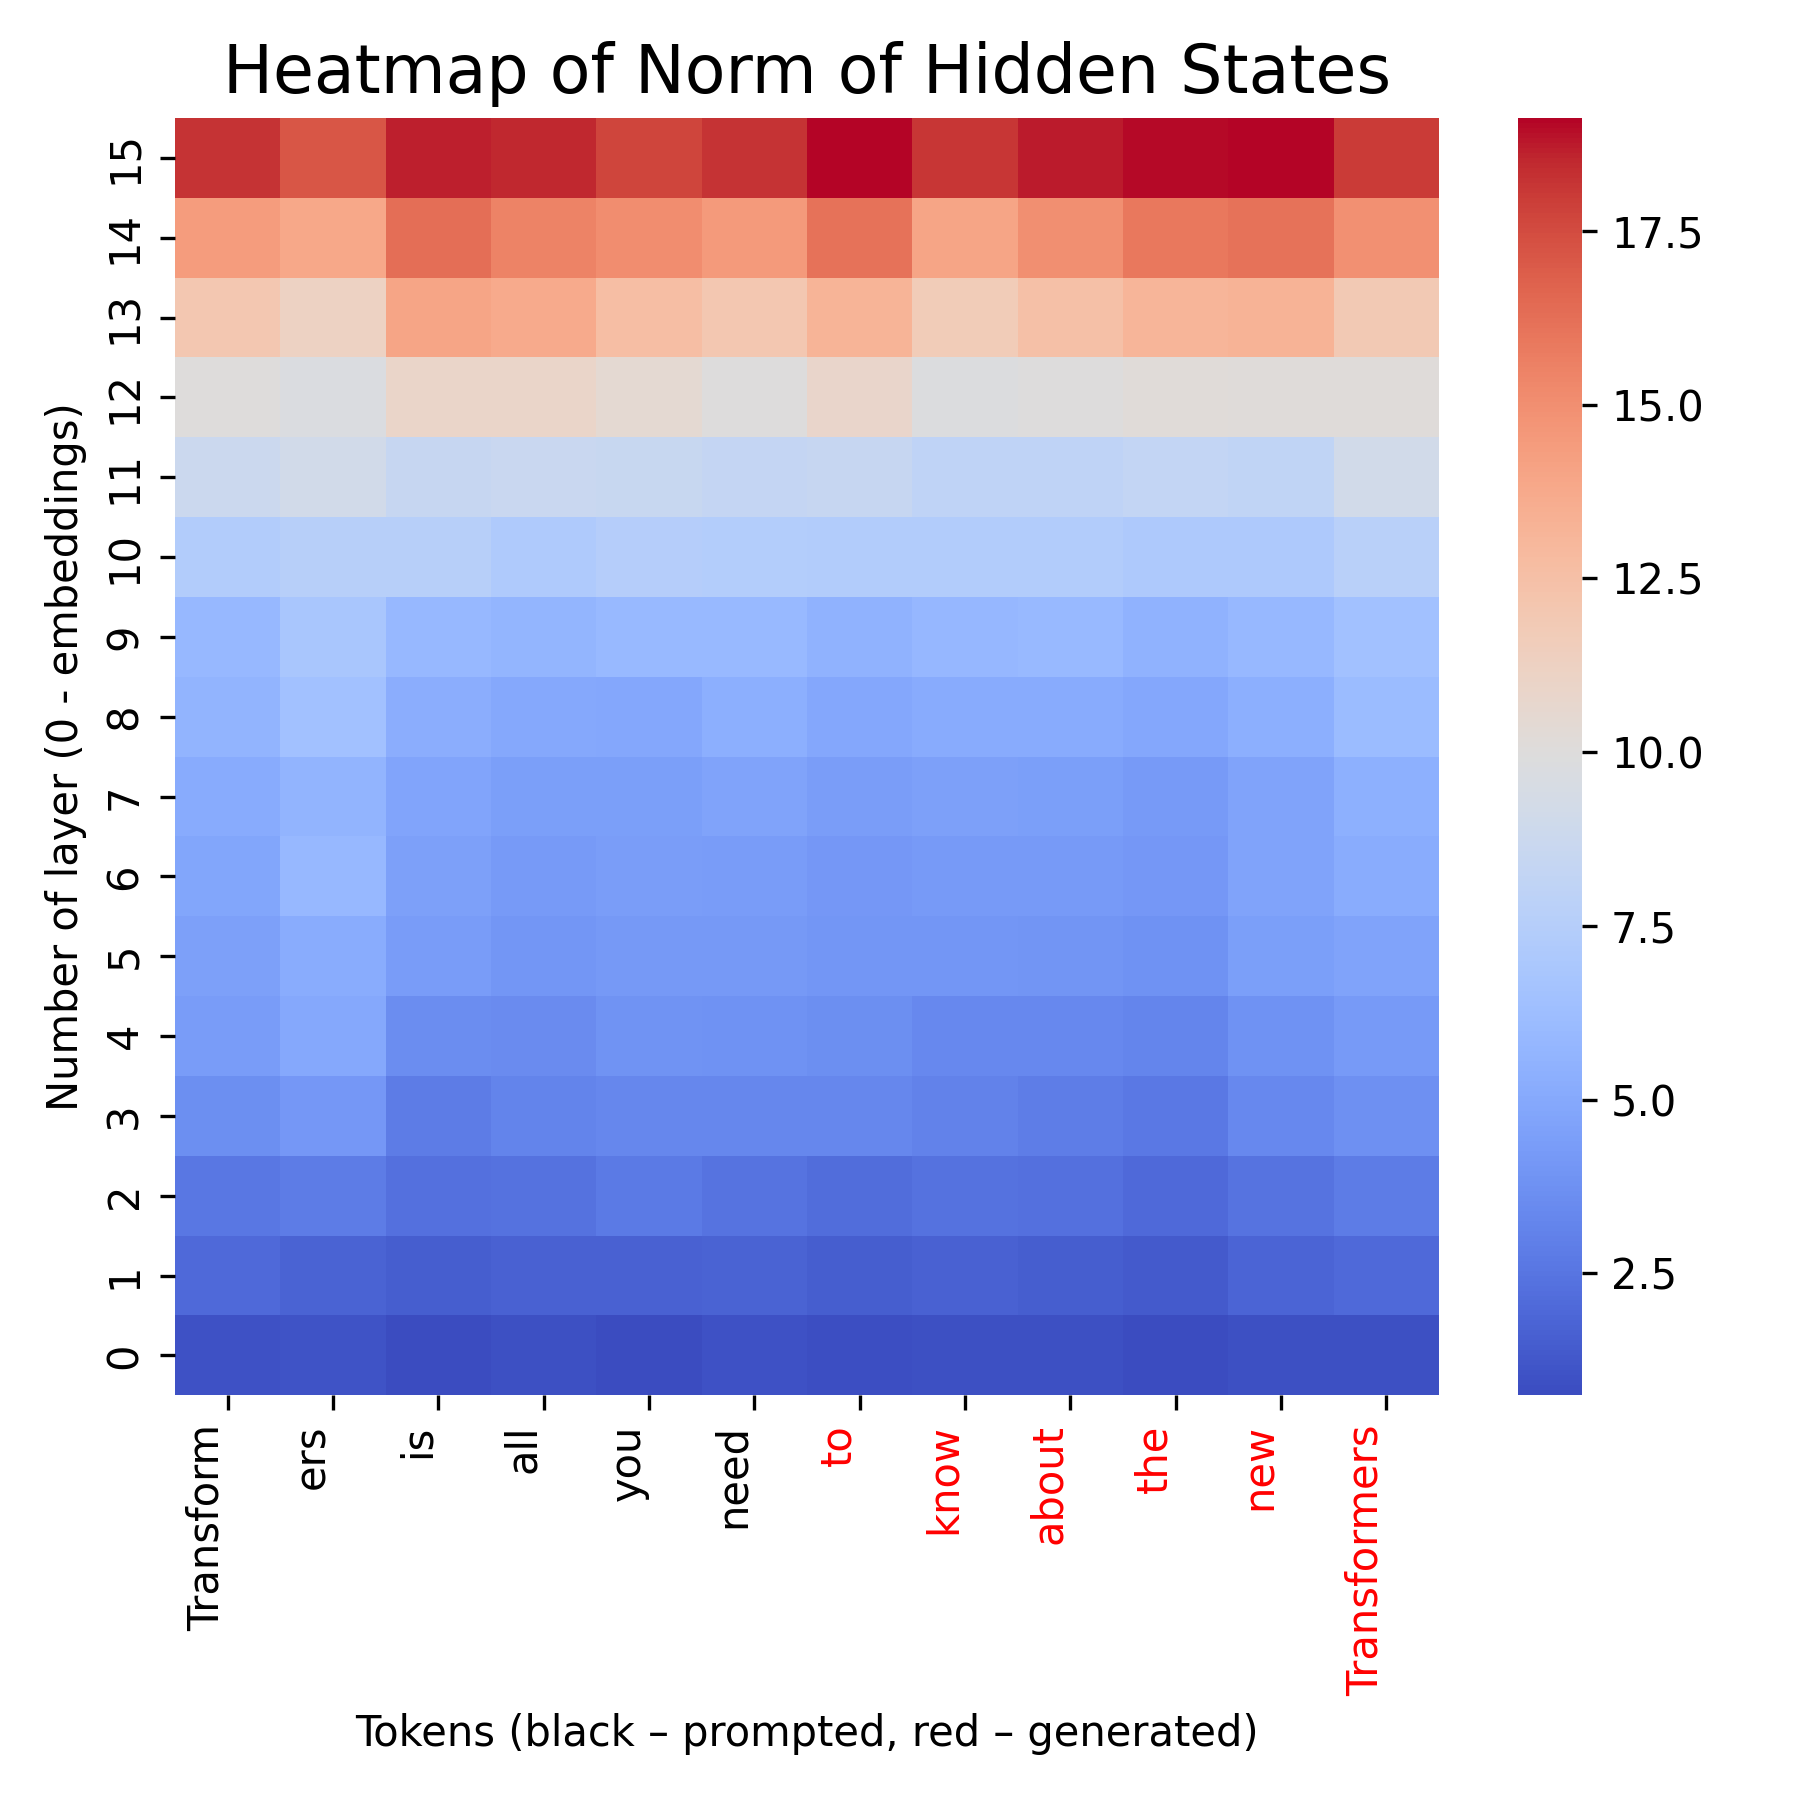
\includegraphics[width=0.5\textwidth]{images/heatmap_1b_notfull.png}
    \caption{Illustration of the k-nearest neighbors approach to token prediction. The final hidden state $\mathbf{h}_i^L$ (blue point) is compared to all token embeddings in the vocabulary. The closest embeddings (green points) correspond to the most likely next tokens, while distant embeddings (red points) are less probable candidates.}
    \label{fig:heatmap_1b_notfull}
\end{figure}


На изображении \ref{fig:heatmap_1b_full} и \ref{fig:heatmap_1b_notfull} можно увидеть heatmap для Llama 3.2 1B. На вход модели подавался промпт "Transformers is all you" и модель сгенерировала по нему 8 токенов (сгенерированные токены отмечены красным цветом). 

Анализируя эти heatmap-ы можно прийти к следующим выводам:
\begin{enumerate}
    \item Промежуточные hidden state для <BOS> токена почти сразу становятся большой нормы. Это явно отличает <BOS> токен от всех остальных.
    \item Hidden state после финального слоя также обладают заметно большей нормой чем все остальные. Это странно.
    \item Если исключить из heatmap колонку для <BOS> токен и строку для последнего hidden state, то можно заметить, что норма hidden state явно растет по мере увелечения номера слоя. При этом нормы ембеддингов токенов (строчка 0 в heatmap) лежат в районе 1. Также не видно разницы между сгенерированными токенами и токенами контекста. Все это показывает нам, что промежуточные hidden state в Llama 3.2 1B выходят далеко за пределы облака точек ембеддингов токенов.
\end{enumerate}


Также мы дополнительно обучили маленькую Llama-like модели с 150M параметров с KnnHead и регуляризатором штрафующим за слишком большое отклонение промежуточных hidden state-ов от облака точек ембеддингов токенов. Подробнее принцип работы этого регуляризатора описан в секции \ref{reg_info}.


% todo сделай две этих картинки параллельно в одну линию через minipage
\begin{figure}[h]
    \centering
    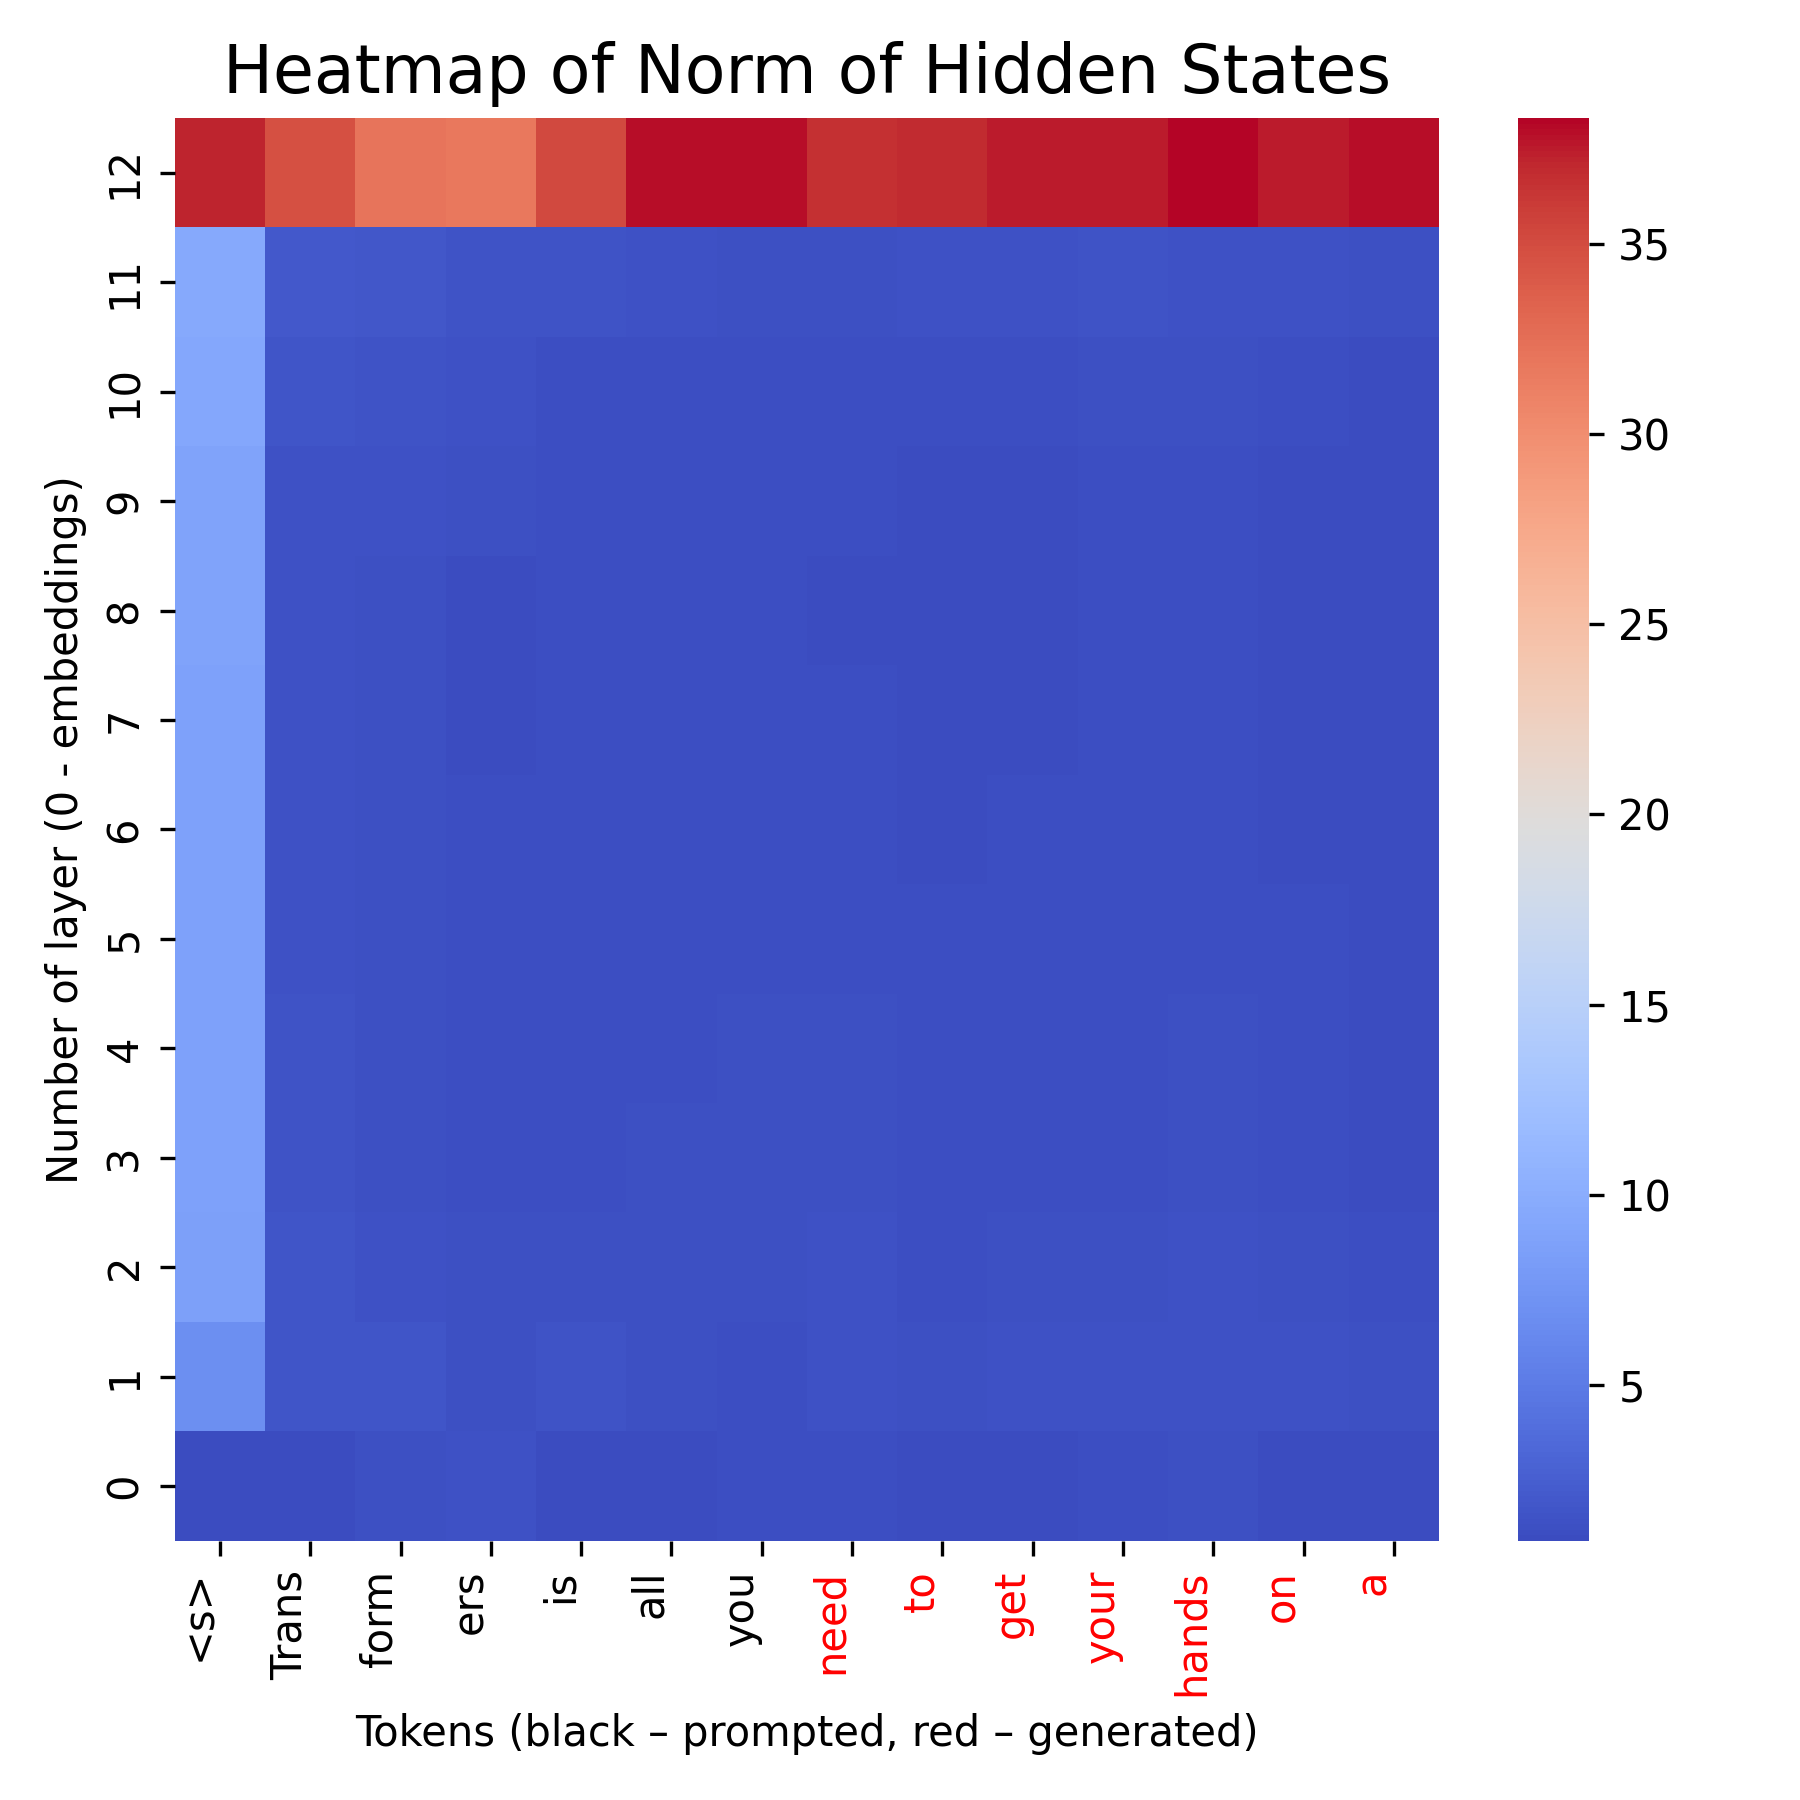
\includegraphics[width=0.5\textwidth]{images/heatmap_150m_reg_all.png}
    \caption{Illustration of the k-nearest neighbors approach to token prediction. The final hidden state $\mathbf{h}_i^L$ (blue point) is compared to all token embeddings in the vocabulary. The closest embeddings (green points) correspond to the most likely next tokens, while distant embeddings (red points) are less probable candidates.}
    \label{fig:heatmap_150m_reg_all}
\end{figure}

\begin{figure}[h]
    \centering
    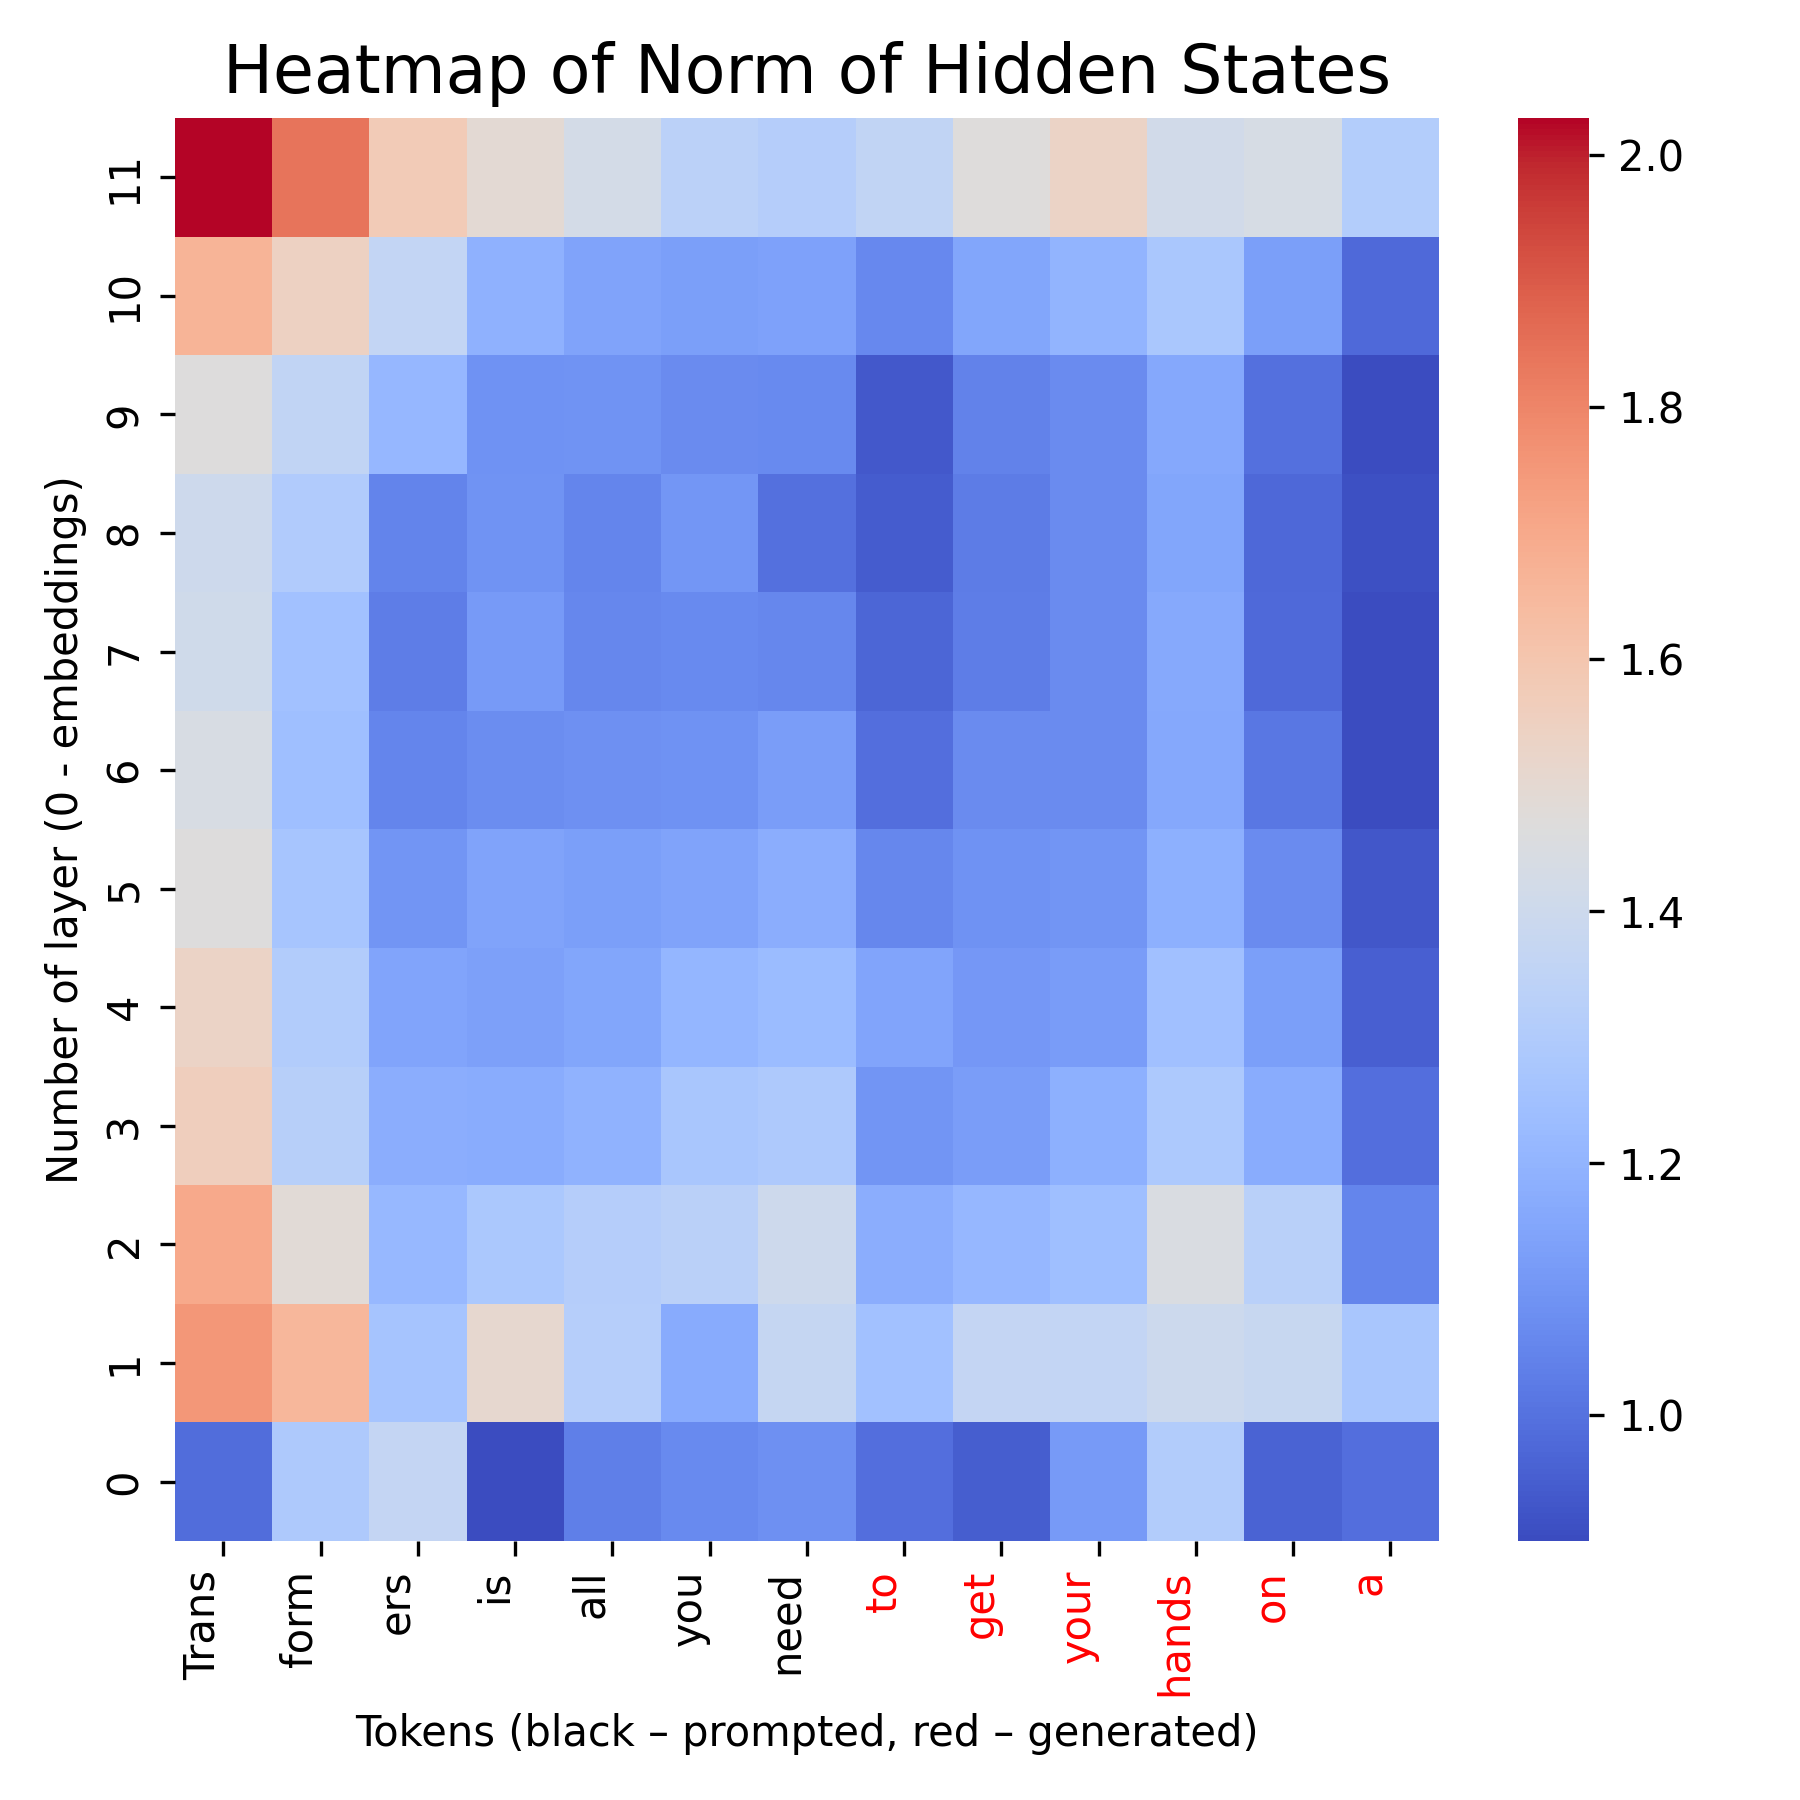
\includegraphics[width=0.5\textwidth]{images/heatmap_150m_reg_notall.png}
    \caption{Illustration of the k-nearest neighbors approach to token prediction. The final hidden state $\mathbf{h}_i^L$ (blue point) is compared to all token embeddings in the vocabulary. The closest embeddings (green points) correspond to the most likely next tokens, while distant embeddings (red points) are less probable candidates.}
    \label{fig:heatmap_150m_reg_notall}
\end{figure}

Из heatmap \ref{fig:heatmap_150m_reg_all} и \ref{fig:heatmap_150m_reg_notall} можно сделать вывод, что регуляризатор справился со своей задачей и промежуточные токены действительно находятся в облаке точек эмбеддингов токенов, так как их нормы сравнимы. При этом ситуация с большыми нормами hidden state-ов <BOS> токена и нормами hidden state-ов после последнего слоя не исправилась. 

Отдельно стоит добавить, что метрики бенчмарков и loss на валидации у модели обученной с таким регуляризатор значительно не изменились. Это можно увидеть на таблице \ref{TODO}